
\newpage
\section{Introducción}
\label{sec:Introduction}

\justifying \setlength{\parindent}{1.27cm}
\normalsize\mdseries

%   Definición del problema
El calentamiento global, la contaminación y la deforestación son conceptos plenamente conocidos y, lamentablemente, constantemente visibles en los medios de actualidad. Todos ellos afectan gravemente a las reservas de agua potable, o de uso en cultivos, del planeta, y por tanto, a la esperanza de vida humana.\newline

En Castilla-La Mancha, nuestra tierra, 7.946.198 hectáreas de terreno son dedicadas al cultivo, y sólo en 474.910 de ellas se despliegan viñedos, sin tener en cuenta las diferentes variedades de uva que los agricultores manchegos pueden o no cultivar (\cite{gob.miapa.01}). Para aprovisionar estos terrenos, se necesita un gran volumen de agua, el cual puede proceder de embalses, aguas depuradas, o acuíferos. Sin embargo, y precedida por los factores perjudiciales para el medio ambiente mencionados al inicio de este documento, la gestión de agua ante eventos extremos, por ejemplo sequías, será cada vez más importante.\newline

%   Descripciones de soluciones actuales
En la actualidad, el sector agrario emplea distintas técnicas de riego para el suministro de agua. Según el \cite{ine.01}, el agua utilizada para riego en España se despliega en las siguientes opciones:

\begin{figure}[h]
    \centering
    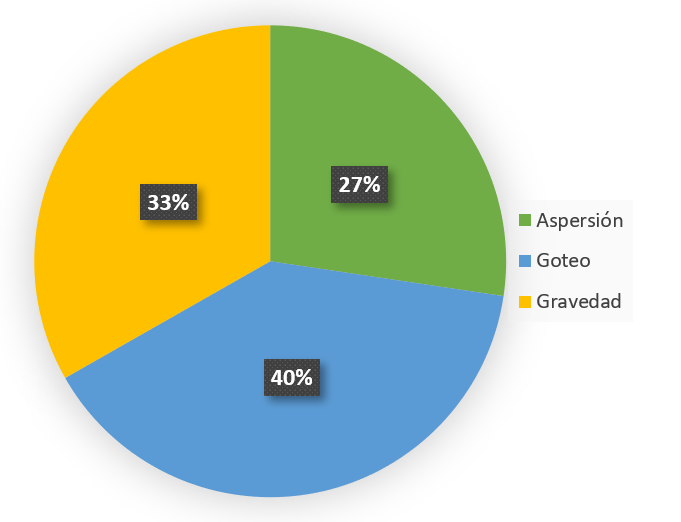
\includegraphics[scale=0.75]{figures/graphics/riego_graphic.png}
    \caption{Sistemas de riego utilizados en España.}
    \label{fig:riego_graphic}
\end{figure}

Actualmente se encuentran varias soluciones en el mercado como la aspersión, el riego por goteo o sistemas de riego automáticos dentro de invernaderos para el suministro de agua. Sin embargo, todos éstos funcionan dentro de franjas horarias sin ningún tipo de mecanismo de adaptación al terreno o a las condiciones que lo envuelven.\newline

%   Objetivos (resumen)
Es por ello que, con el fin de reducir al máximo posible el consumo de agua, con razón de cuidado de plantaciones y cultivos, se propone con este proyecto alcanzar una nueva alternativa adaptativa frente a los sistemas de riego convencionales. Para ello, se diseñará e implementará un sistema de control de riego automatizado para porciones de terreno grandes.\newline

%   Descripción de mi solución con figuras etc
La solución optada se compone de dos subsistemas diferenciados:
\begin{enumerate}
    \item Sensores y controladores del caudal del agua ({\bfseries SubLC}): Estos componentes tendrán la tarea de monitorizar los distintos factores medibles del entorno de la plantación (temperatura, humedad del suelo, etc.) y controlar el caudal necesitado por el propio terreno en función de estos.
    \item Servicio en la red ({\bfseries SubI}): Se dispondrá un servicio disponible en la red que mostrará los datos recogidos por SubLC al usuario, y además controlará al sistema SubLC.
\end{enumerate}

Se explorará más a fondo la arquitectura del sistema en el capítulo \ref{sec:target} del presente documento.